%%%%% Description: big-theory-small-system vs. small-theory-big-system %%%%%
%%%%% Date: July 24, 2016 %%%%%
%%%%% Author: Hengfeng Wei (hengxin) %%%%%
%%%%% Note: The egg shape is drawn by [Benedikt Bauer](http://tex.stackexchange.com/a/74175/23098). %%%%% 

\documentclass{standalone}
\usepackage{tikz}
\usetikzlibrary{intersections}

\begin{document}
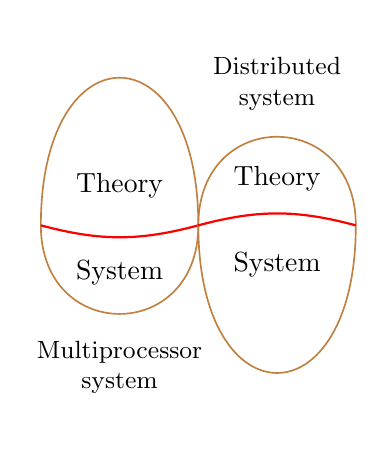
\begin{tikzpicture}

  \begin{scope}[xshift = -4.0cm]
	\draw [semithick, brown, name path = egg] (0,0) 
	  .. controls (0,-1.5) and (2,-1.5).. (2,0)
	  .. controls (2,2.5) and (0,2.5) .. (0,0);

	\draw[thick, red] (0., 0) to [out = -15, in = -165] node[] {} (2, 0);

	\node[] at (1, 0.5) {Theory};
	\node[] at (1, -0.6) {System};

	\node[font = \small, align = center] at (1, -1.8) {Multiprocessor\\system};
  \end{scope}

  \begin{scope}[rotate = 180]
    \draw [semithick, brown, name path = egg] (0,0) 
	  .. controls (0,-1.5) and (2,-1.5).. (2,0)
	  .. controls (2,2.5) and (0,2.5) .. (0,0);

	\draw[thick, red] (0., 0) to [out = -15, in = -165] node[] {} (2, 0);

	\node[] at (1, 0.5) {System};
	\node[] at (1, -0.6) {Theory};

	\node[font = \small, align = center] at (1, -1.8) {Distributed\\system};
  \end{scope}
\end{tikzpicture}
\end{document}
